\begin{figure*}[h!]\centering
  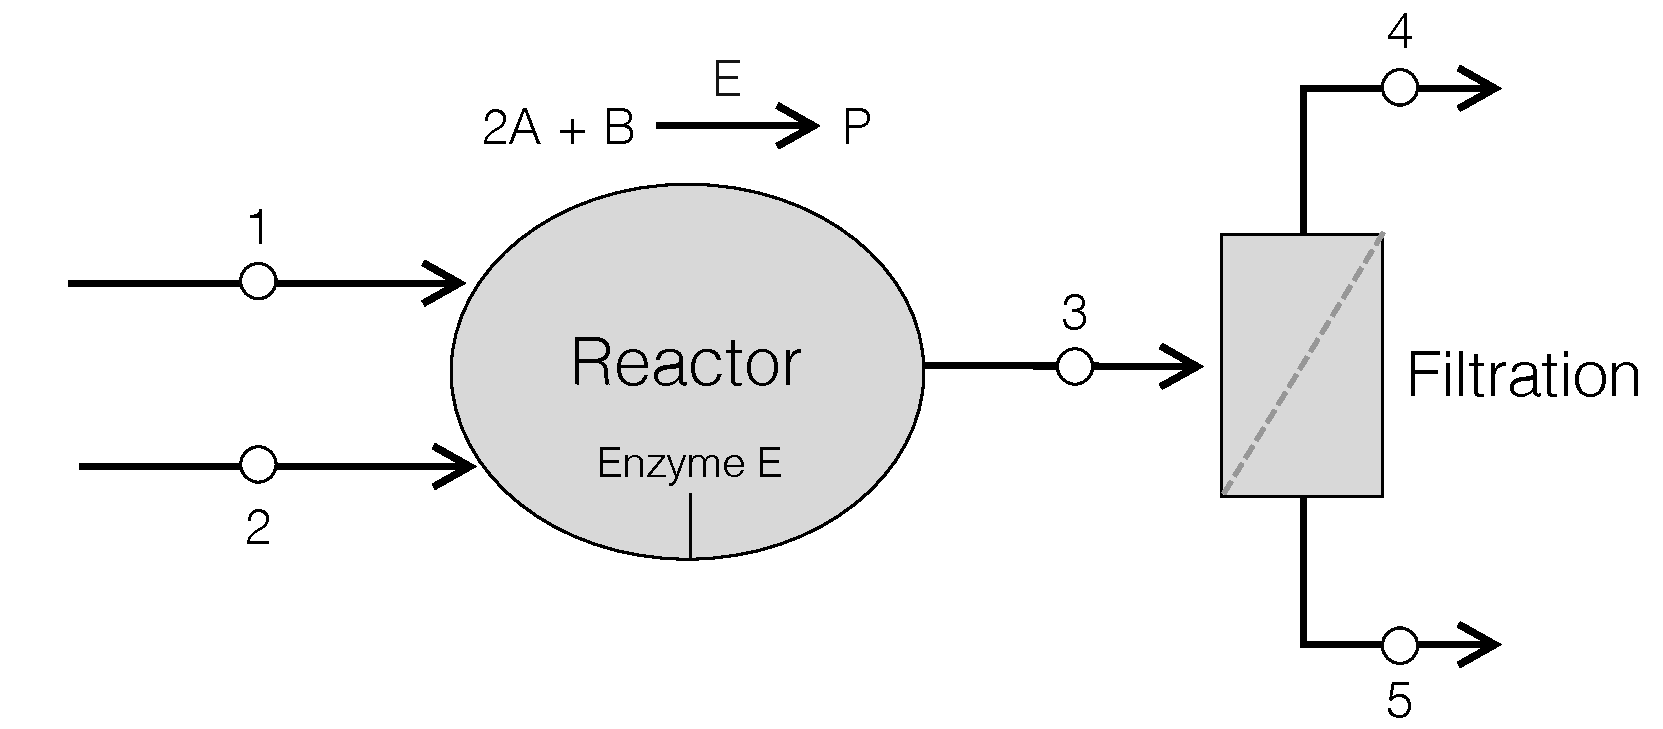
\includegraphics[width=0.80\textwidth]{./figs/Fig-Schematic-Reactor-Problem.pdf}
  \caption{Starting material(s) $A$ and $B$ are converted to product $P$ by enzyme $E$ in a well-mixed reactor with volume $V$. 
  The reactor is well insulated. 
  The output from the reactor is fed into a filtration unit that separates reactants and products.}\label{fig-reactor-splitter}
  \end{figure*}

    \item{(20 pt) Consider the reaction/separation process shown in Fig. \ref{fig-reactor-splitter}.
    In a well-mixed and well-insulated reactor, starting material(s) $A$ and $B$ are converted to the product $P$ by enzyme $E$.
    The enzyme $E$ is immobilized in the reactor (does not flow out) and is stable. Downstream of the reactor,
    a filtration device separates unreacted starting material(s) $A$ and $B$ from product $P$.
   
    \textbf{Assume}: (i) the reactor and filtration units operate at steady-state;
    (ii) let species $(A,B,P)$ have indexes $(1,2,3)$;
    (iii) there is no product in the input streams

    \begin{itemize}
        \item[a)]{~(16 pt)~Compute the missing values in Table \ref{tbl-reactor-filter} if the open extent of reaction $\dot{\epsilon}_{1}$ was measured to be 26.8 mmol min$^{-1}$.}
        \item[b)]{~(2 pt)~Derive an expression for the fractional conversion of species $i$, denoted by $f_{i}\geq{0}$ for the reactor configuration shown in Fig. \ref{fig-reactor-splitter}}. 
        \item[c)]{~(2 pt)~Using the expression from b), compute the fractional conversion for species $A$ and $B$.}

    \end{itemize}
    }


    \clearpage
    
    \begin{table}[!ht]
      \centering
      \caption{State table for the reaction/filtration problem; $\dot{n}_{s,T}$ denotes the total mole flow rate in stream $s$, 
      $x_{s,1}$ denotes the mole fraction of component 1 (A) in stream $s$, 
      $x_{s,2}$ denotes the mole fraction of component 2 (B) in stream $s$, and
      $x_{s,3}$ denotes the mole fraction of component 3 (P) in stream $s$.}\label{tbl-reactor-filter}
    
      \renewcommand{\arraystretch}{2.0}
      \setlength{\tabcolsep}{14pt}
      \begin{tabular}{c|c|c|c|c}\toprule
      Stream $i$ & $\dot{n}_{s,T}$ (mmol/min) & $x_{s,1}$ & $x_{s,2}$ & $x_{s,3}$ \\ \bottomrule
      1 & 95 & 1.0 & 0.0 & 0.0 \\ \hline
      2 & 45 & 0.11 & 0.89 & 0.0   \\ \hline
      3 & & & &   \\ \hline
      4 & & & & \\ \hline
      5 & 59.54 & 0.77 & 0.22 & 0.01 \\ \bottomrule
      \end{tabular}
    \end{table}